\documentclass[a4paper,fleqn]{cas-sc}

\usepackage[authoryear,longnamesfirst]{natbib}
\usepackage{amsmath,amssymb}
\graphicspath{{./}{../}}   % figures live in ../figs when compiling from report/

\ExplSyntaxOn
\cs_set:Npn \__first_footerline:
  { \group_begin: \small \sffamily \__short_authors: :~ { \rmfamily \itshape Supplementary~Material } \group_end: }
\ExplSyntaxOff
\RenewDocumentCommand\printorcid{}{}

\renewcommand{\thefigure}{S\arabic{figure}}
\renewcommand{\thetable}{S\arabic{table}}

\begin{document}
\let\WriteBookmarks\relax

\shorttitle{Neural Parameter Estimation for Discrete Bayesian Networks: Supplementary Material}
\shortauthors{K. Aspoas}

\title [mode = title]{Supplementary Material: Neural Network Parameter Estimation for Discrete Bayesian Networks with Applications in Medical Diagnosis}

\author[1]{Kaylin Aspoas}
\affiliation[1]{organization={School of Computer Science and Applied Mathematics, University of the Witwatersrand},
            city={Johannesburg},
            country={South Africa}}

\begin{abstract}
This document contains supplementary figures and tables referenced in the main report. Supplementary Figures~S1 and S2 and Supplementary Table~S1 support the architecture selection results, and Supplementary Figure~S3 shows the expert-elicited structure used in the real-data experiments.
\end{abstract}

\maketitle

\begin{figure}[h]
\centering
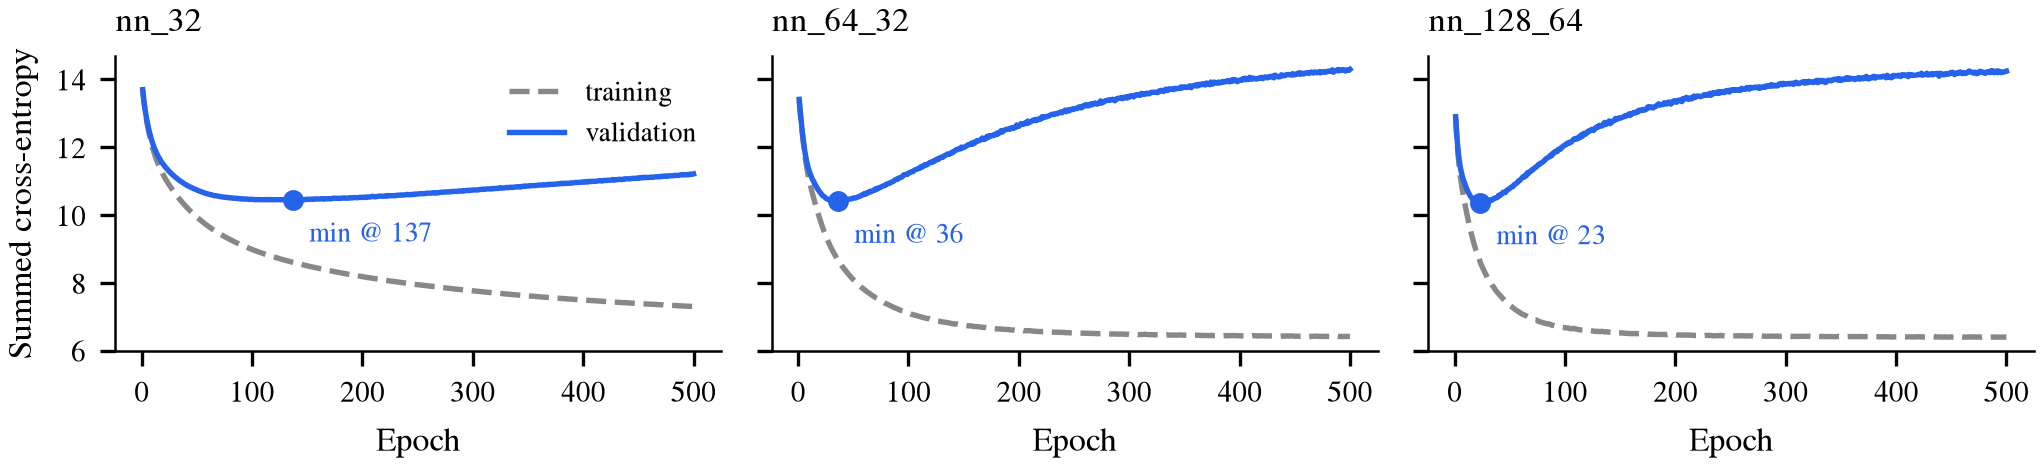
\includegraphics[width=\textwidth]{figs/no_es.png}
\caption{Summed training and validation cross-entropy without early stopping ($r=2$, $k=10$, $N=600$, mean over five tuning DAGs). The marker shows the lowest validation loss.}\label{fig:noes}
\end{figure}

\begin{figure}[h]
\centering
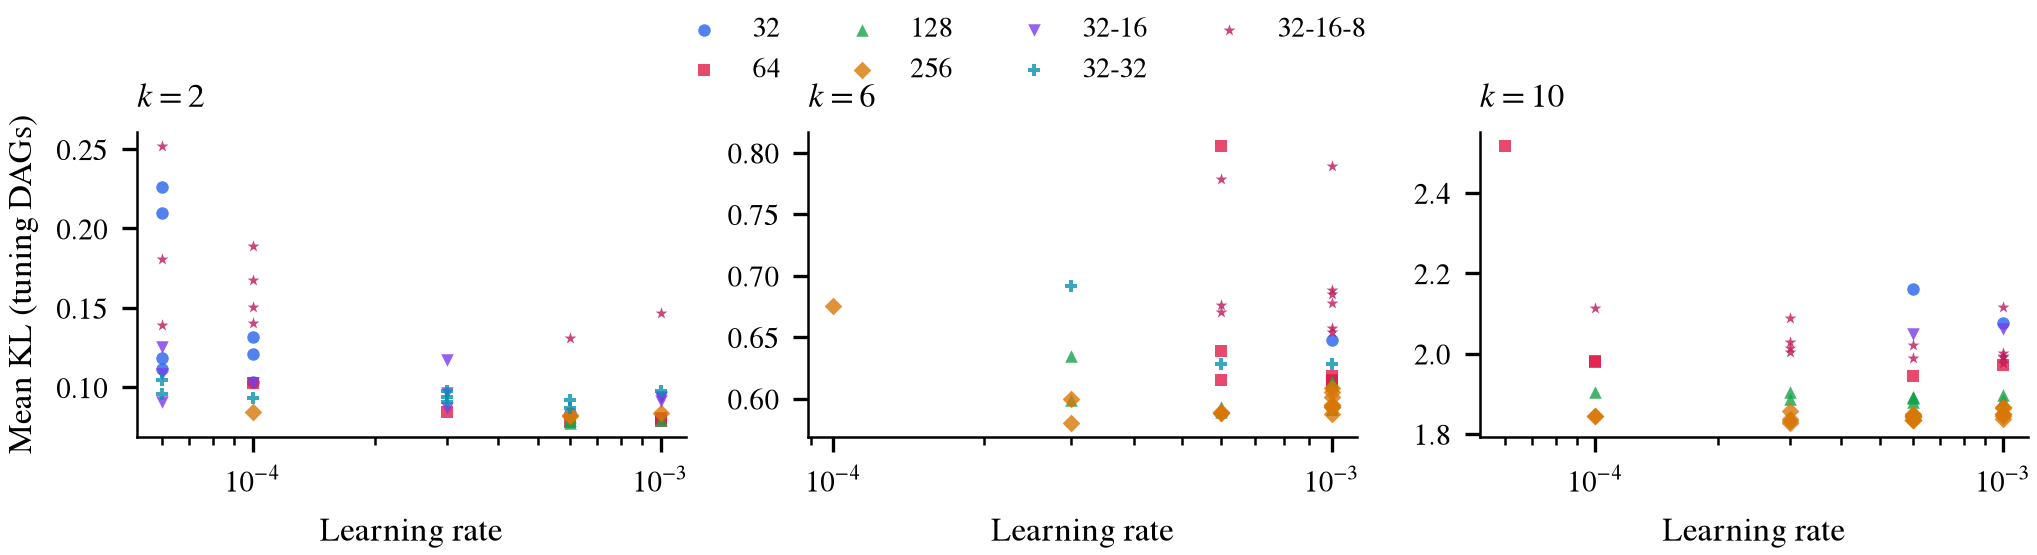
\includegraphics[width=\textwidth]{figs/sweep_c2.png}
\caption{Bayesian hyperparameter sweeps ($r=2$). Each point is one trial's mean KL over five tuning DAGs and two sample sizes; colour indicates the hidden layers (log-scaled x-axis).}\label{fig:sweep}
\end{figure}

\begin{table}[h]
\caption{Chosen configurations for $r=4$: mean validation loss over five tuning DAGs. All configurations fall within three standard errors of the best at every setting.}\label{tab:cand}
\small\setlength{\tabcolsep}{3pt}
\begin{tabular*}{\tblwidth}{@{\extracolsep{\fill}}lrrrrrrrrr@{}}
\toprule
 & \multicolumn{2}{c}{$k=2$} & \multicolumn{2}{c}{$k=6$} & \multicolumn{2}{c}{$k=10$} & & & \\
Configuration & $N{=}600$ & $N{=}1400$ & $N{=}600$ & $N{=}1400$ & $N{=}600$ & $N{=}1400$ & lr & Dropout & Batch \\
\midrule
\texttt{nn\_256} & 17.66 & 17.45 & 24.79 & 24.21 & 24.87 & 24.50 & $6{\times}10^{-4}$ & 0.0 & 32 \\
\texttt{nn\_128\_64} & 17.60 & 17.41 & 24.77 & 24.20 & 24.81 & 24.45 & $6{\times}10^{-4}$ & 0.3 & 32 \\
\texttt{nn\_64\_32} & 17.65 & 17.46 & 24.77 & 24.16 & 24.85 & 24.47 & $6{\times}10^{-4}$ & 0.3 & 32 \\
\texttt{nn\_32\_16} & 17.76 & 17.57 & 24.80 & 24.25 & 24.87 & 24.51 & $10^{-3}$ & 0.3 & 32 \\
\texttt{nn\_32} & 17.79 & 17.58 & 24.88 & 24.42 & 24.95 & 24.61 & $6{\times}10^{-4}$ & 0.3 & 64 \\
\bottomrule
\end{tabular*}
\end{table}

\begin{figure}[h]
\centering
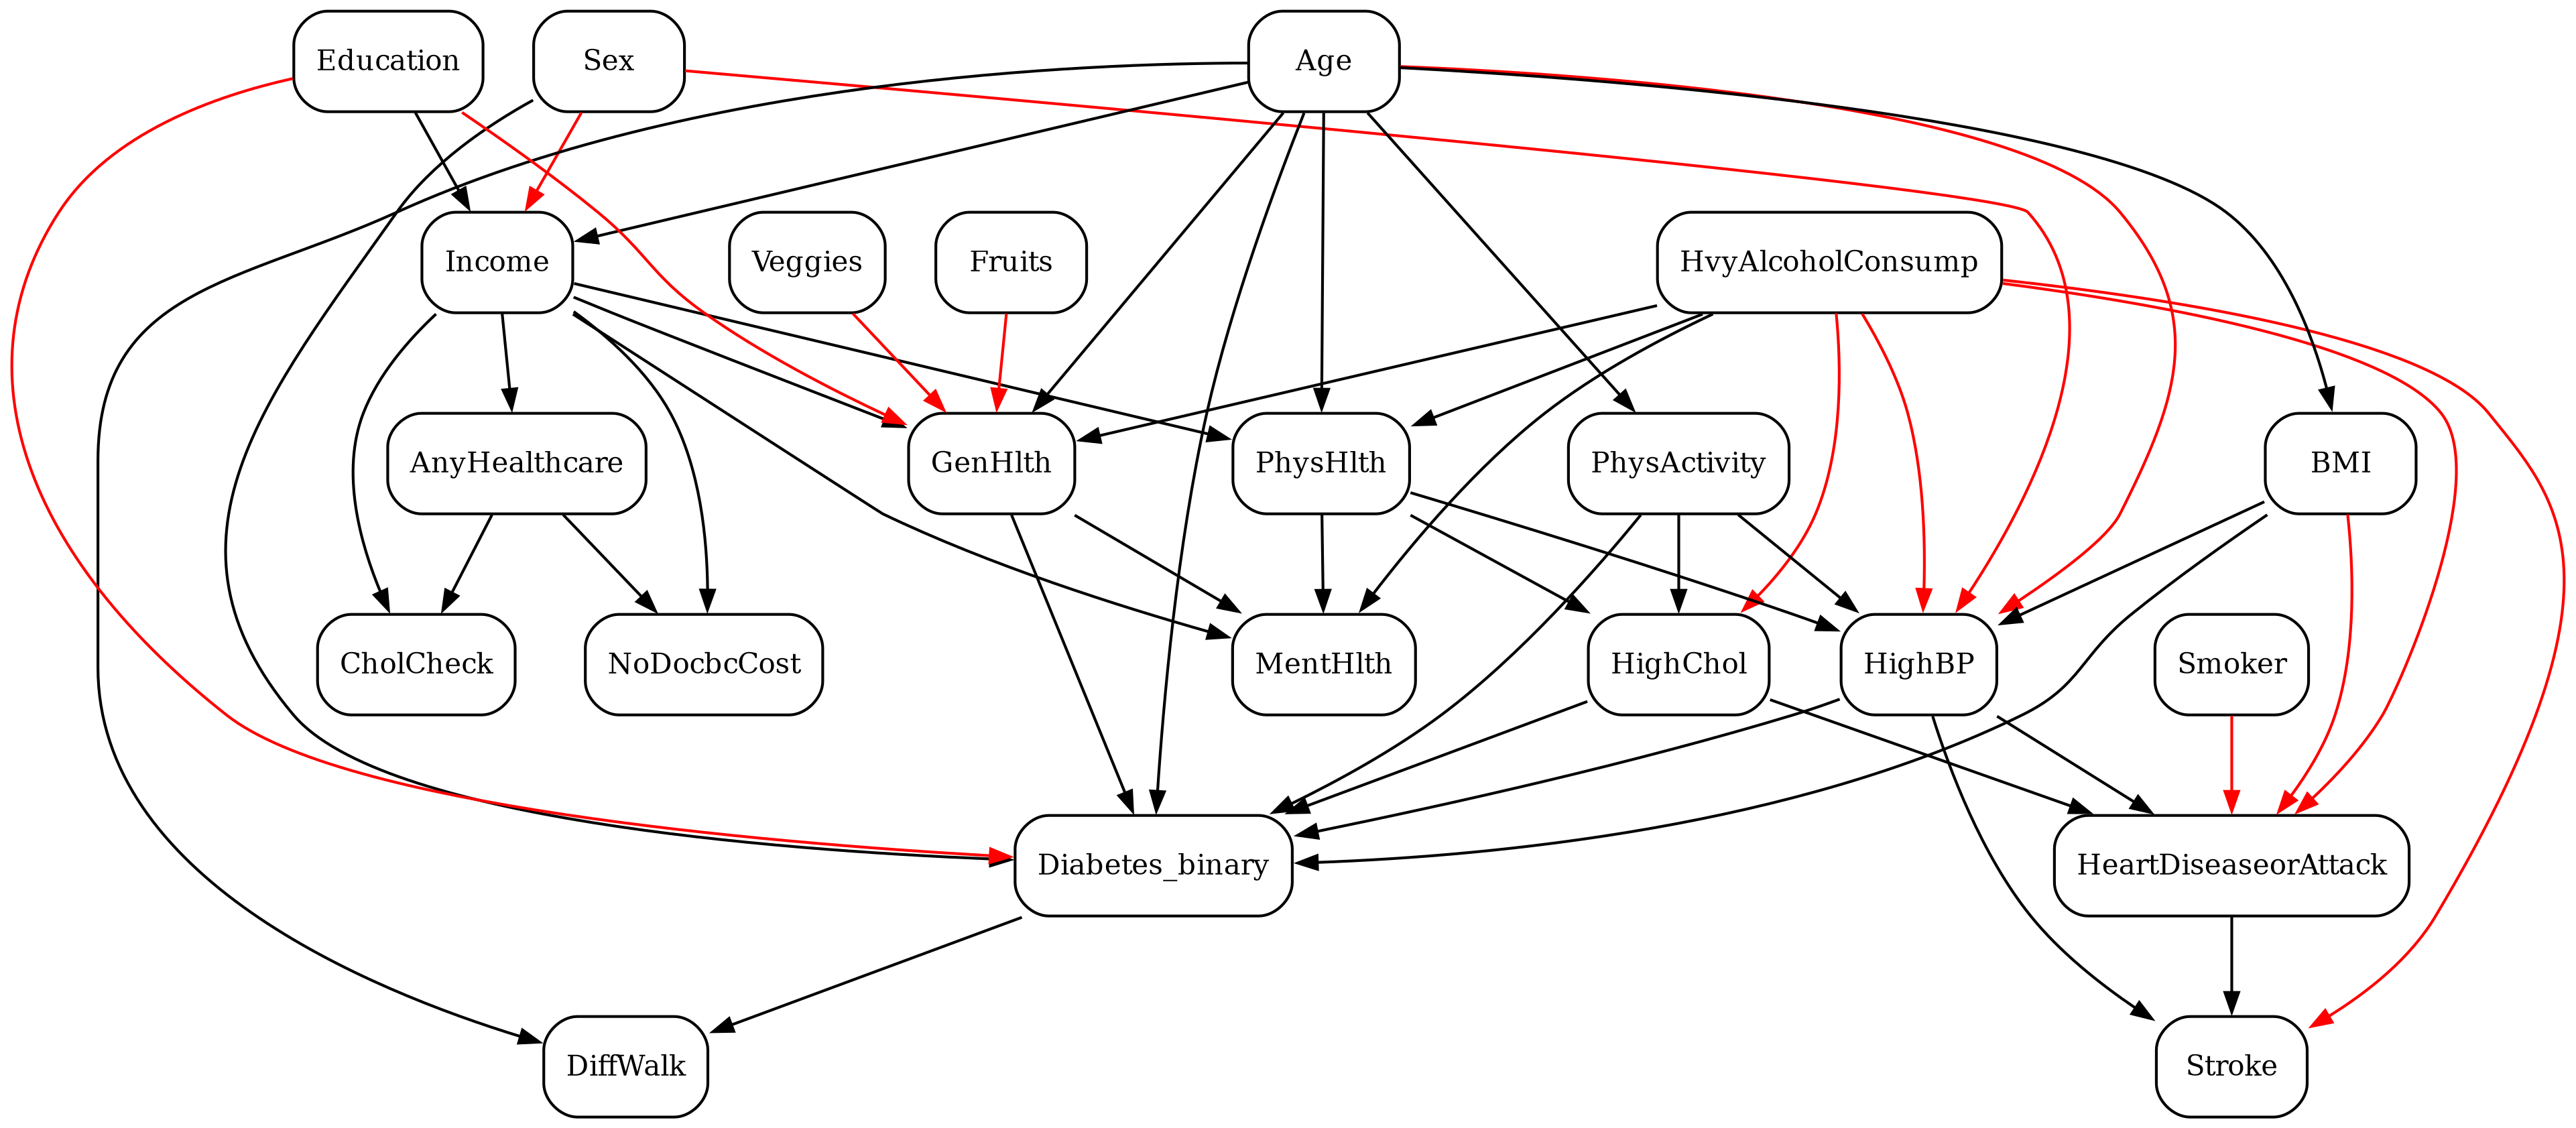
\includegraphics[width=0.82\textwidth]{figs/dag_moderate.png}
\caption{Moderate-confidence expert DAG for the CDC Diabetes Health Indicators data \citep{zahoor2025investigatingvaliditystructurelearning}. Black edges form the high-confidence DAG; red edges are added at moderate confidence.}\label{fig:dag}
\end{figure}

\begin{figure}[h]
\centering
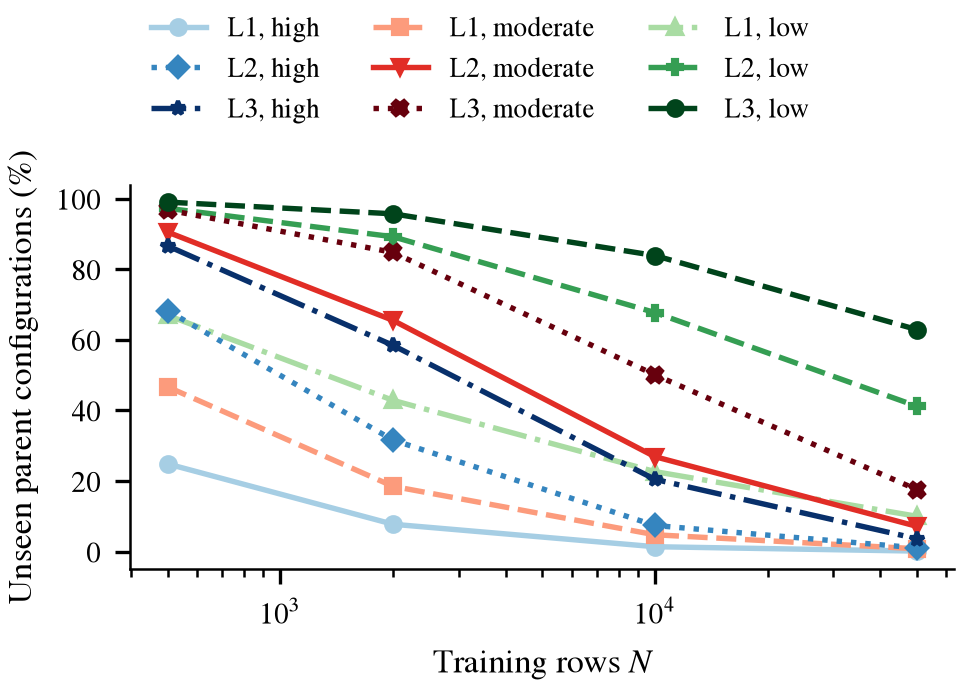
\includegraphics[width=\textwidth]{figs/real_unseen.png}
\caption{Percentage of test rows in which at least one node's parent configuration never occurs in the training data, for each discretisation and DAG combination (log-scaled x-axis).}\label{fig:unseen}
\end{figure}

\bibliographystyle{cas-model2-names}
\bibliography{references}

\end{document}
